\chapter*{Introducción}\label{chapter:introduction}
\addcontentsline{toc}{chapter}{Introducción}

Cuba se ha propuesto, desde hace unos años, llevar a cabo un profundo proceso de informatización.
Entre los temas dentro de dicho proceso, que tienen como objetivo facilitar muchas actividades
cotidianas, se encuentran: transacciones bancarias, comercio electrónico, mayor acceso a internet, digitalización
de información, acceso a información, etc. Una de las tantas actividades que desde hace ya tiempo se ha convertido en
cotidiana, es el uso de los medios de transporte terrestres para desplazar mercancías o personas de un lugar a otro de
manera más rápida. Para esto se han ido desarrollado las carreteras, y se han ido mejorando con materiales para facilitar
el desplazamiento y a la vez hacerlas más resistentes. Aún así, en los tiempos actuales las carreteras se deterioran
debido al clima, al tráfico o a la mala calidad de los distintos tipos de trabajo que se llevan a cabo en la vía
pública. En Cuba es algo bastante común que la mayoría de las carreteras en las grandes ciudades, como La Habana,
estén en malas condiciones.\\

\begin{figure}[htb]
	\centering
	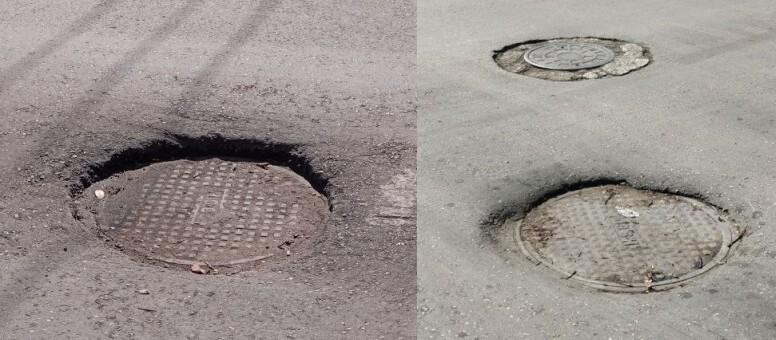
\includegraphics[scale=0.45]{Graphics/pothole_due_to_bad_job_1}
	\caption{Baches ocasionados por trabajos de reparación mal ejecutados.}
	\label{fig:1}
\end{figure}

\indent El acceso rápido a la ubicación de los tramos de carretera en mal estado sería muy útil, pues no solo permitiría agilizar la
reparación de estas calles, sino que también podría servir de guía a choféres para evitar tales tramos. Esto evitaría las posibles
consecuencias ocasionadas por estas condiciones, como accidentes y daños a la estructura de los vehículos. Además, el hecho de no tener que
enviar vehículos a inspeccionar el estado de las carreteras, constituye un ahorro importante de recursos y de tiempo. De esta forma se podrían
tomar decisiones con mayor rapidez sobre que tramos de carretera priorizar.\\
\indent Muchos de los primeros trabajos que se propusieron resolver el problema de determinar los tramos de carreteras en mal estado, utilizaban
métodos de detección que se basaban en fijar umbrales, y que a pesar de funcionar no tenían muy buena precisión ~\brackcite{eriksson2008pothole,
mohan2008nericell, mednis2011real}. Más recientemente con el auge del aprendizaje de máquinas muchos autores han atacado este problema utilizando
las bondades de dicha rama, extrayendo varios \emph{features} de dominio temporal y de frecuencia, y utilizando métodos como \emph{Support Vector
Machines} (\textbf{SVM}), redes neuronales artificiales(\textbf{ANN}) y árboles de decisión (\textbf{DT}) ~\brackcite{el2018towards, seraj2015roads,
gonzalez2017learning, zheng2020fused, perttunen2011distributed}. Muchos autores han tenido en cuenta además la naturaleza contaminada por ruido de
los datos obtenidos utilizando estos dispositivos y han utilizando técnicas de procesamiento de señales digitales para mejorar la calidad de la señal
obtenida con el objetivo de obtener datos más significativos que caractericen de forma más precisa la señal y por lo tanto mejoren la calidad de las
predicciones de los modelos de \emph{Machine Learning} ~\brackcite{el2018towards, zheng2020fused, perttunen2011distributed, gonzalez2017learning}.\\
\indent En la isla no se conoce ninguna forma de ubicar de forma sencilla y accesible los tramos de carreteras que están en mal estado. Una herramienta
que pudiera facilitar esta información podría contribuir a mejorar el estado de los viales en La Habana, y a mantener a las autoridades y a los choferes
al tanto de las condiciones de las calles. Además, el grupo de Inteligencía Artificial de \textbf{MATCOM} está interesado en contribuir a una posible
solución de este problema, y aún no tiene una línea de investigación dedicada a intentar resolver esta cuestión.\\
\indent Para resolver este problema se explorará la factibilidad de un modelo de aprendizaje de máquinas para detectar y clasificar las anomalías en la
carretera de forma automática. Los datos serán obtenidos de los sensores integrados en un dispositivo móvil, como el \textbf{acelerómetro},
el \textbf{giroscopio} y el \textbf{GPS}.\\
\indent El objetivo general de este trabajo es proponer un modelo para la detección de baches utilizando los sensores embebidos en los
dispositivos móviles. Para lograr esto se pretende:

\begin{itemize}
	\item Estudiar el estado del arte del uso de Dispositivos Móviles para la Detección de Baches.
	\item Determinar el conjunto de sensores apropiados para la detección de baches, así como su frecuencia de muestreo.
	\item Implementar un prototipo de aplicación para la captura de los datos de los sensores, así como la señalización
		manual de baches.
	\item Proponer e implementar un modelo para la detección automática de baches.
	\item Proponer e implementar un prototipo para la visualización de los datos.
	\item Proponer una metodología para validar los resultados parciales.
\end{itemize}

\indent La propuesta en cuestión se basa en los datos que se obtienen con el \textbf{acelerómetro}, el \textbf{giroscopio} y el \textbf{GPS}, que
son sensores que permiten obtener los datos de la aceleración, la velocidad de giro y la geolocalización del dispositivo móvil respectivamente.
Con esta información pudiera ser viable implementar un modelo de aprendizaje de máquinas que sea capaz de detectar de forma automática los baches
en la carretera y ubicarlos en un mapa. Existen varias razones por las que se propone utilizar los dispositivos móviles actuales en la propuesta:\\

\begin{itemize}
	\item Tener acceso a los sensores de forma independiente es complicado, y lograr una configuración y sincronización de los mismos también lo es.
	\item En la mayoría de los dispositivos móviles estos sensores vienen integrados, lo que facilita la recolección de información.
	\item Cada vez se hace más común que gran parte de las personas tengan un dispositivo móvil y lo usen para realizar distintas actividades.
		Esto permite que sus dispositivos puedan ser utilizados para obtener los datos necesarios a partir de las lecturas que se obtienen de los
		sensores que tienen integrados. Por lo que muchas personas podrían contribuir en la recolección de datos para mejorar la propuesta.
\end{itemize}
